\documentclass[10pt]{article}
\usepackage[a4paper, left=1.5cm, right=1.5cm, top=3.5cm]{geometry}
\usepackage[ngerman]{babel}
\usepackage[]{graphicx}
\usepackage{multicol}
\usepackage{amssymb}
\usepackage{inputenc}
\usepackage{breqn}
\usepackage{titlesec}
\usepackage{wrapfig}
\usepackage{blindtext}
\usepackage{lipsum}
\usepackage{caption}
\usepackage{listings}
\usepackage{fancyhdr}
\usepackage{nopageno}
\usepackage{authblk}
\usepackage{amsmath}
\usepackage{mathtools}
\usepackage{bm}
\usepackage[ISO]{diffcoeff}
\usepackage{xcolor}
\usepackage{csquotes}
\usepackage{siunitx}
\usepackage{circuitikz}
\fancyhf[]{}

\newenvironment{Figure}
  {\par\medskip\noindent\minipage{\linewidth}}
  {\endminipage\par\medskip}

\begin{titlepage}
    \title{Elektronikpraktikum -- Versuch 8: Mikroprozessor}
    \author[1]{Jonas Wortmann\thanks{s02jwort@uni-bonn.de}}
    \author[1]{Angelo V. Brade\thanks{s72abrad@uni-bonn.de}}
    \affil[1]{Rheinische Friedrich-Wilhelms-Universität Bonn}
    \date{\today}
\end{titlepage}

\begin{document}
\pagenumbering{gobble}
\maketitle
\newpage

\tableofcontents
\newpage

\pagenumbering{arabic}

\pagestyle{fancy}
\fancyhead[R]{\thepage}
\fancyhead[L]{\leftmark}


\begin{multicols}{2}
	\section{Einleitung}
  In diesem Versuch werden wir einen Prozessor angefangen von einigen wenigen logischen Verknüpfunkt bis zu einem vollständig mit Assambly programmierbaren 8080 Mikroprozessor verstehen. Dafür wird zunächst die Arithmetic Logic Unit und dann dessen Ereweiterungen betrachtet. Zum Schluss führen wir ein Programm zu Multiplikation von Zahlen aus.
	\section{Theorie}
  \subsection{Grundlagen}
  Als Grundlage unserer logischen Operationen dient, wie schon zuvor untersucht und verstanden, die Binärarithmetik. Es lassen sich z.B. Zahlen einfach addieren, wobei auf ein Überlauf geachtete werden muss. Ein Überlauf dritt dann auf, wenn das Ergebnis größer, als die Speichergröße der Zahl ist. Es lässt sich auch eine Subtraktion durch umwandlung des Subtrahenden in eine Addition überführen. Dafür wird der Subtrahend bitweise invertiert und von dem gesammten Subtrahenden 1 abgezogen. Im allgemeinen lassen sich mit Binärzahlen aber genauso rechnen, wie wenn man die Dezimalbasis, statt der Binärbasis, benutzt. Neben den Binärzahlen werden auch Hexadezimalzahlen verwendet, da diese sich mit genau 4 Bits darstellen lassen. Durch die verkürtzte schreibweise werden sie zur Datenspeicherung verwendet. So können auch zwei Hexadezimalzahlen einen Byte (8 Bit) bilden. 
  \subsection{Arithmetic Logic Unit}
  Die Arithmetic Logic Unit (Abb. \ref{fig:alu}), kurz ALU, ermöglich die Verknüpfung von AND, OR und XOR, sowie die Verknüpfungen des integrierten 8-Bit-Addier-Subtrahierwerks (Abb. \ref{fig:addsub}). 
  \begin{Figure}
    \centering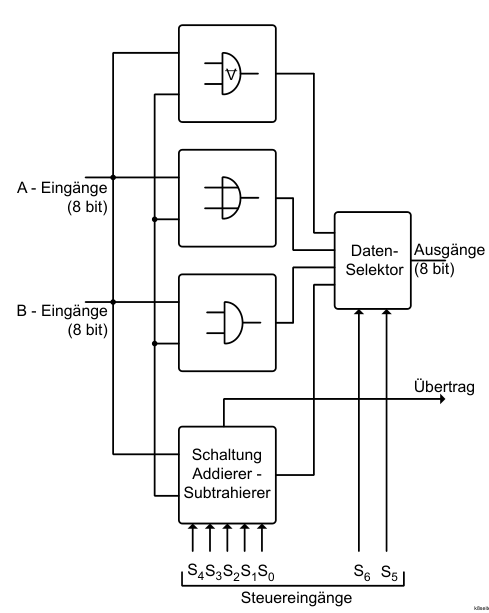
\includegraphics[width=0.8\textwidth]{alu.png}
    \captionof{figure}{Arithmetic Logic Unit}
    \label{fig:alu}
  \end{Figure}
  \begin{Figure}
    \centering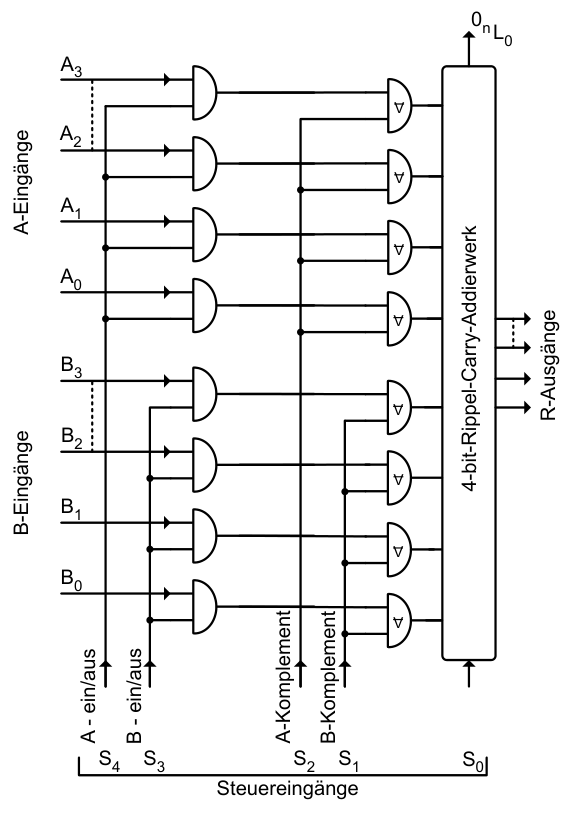
\includegraphics[width=0.7\textwidth]{addier-subtrahierwerk.png}
    \captionof{figure}{8-bit Addier-Subtrahierwerk}
    \label{fig:addsub}
  \end{Figure}

  \subsection{Akkumulator}
  Erweitert man den ALU mit einem ROM, sowie einem Register und einer Übertragsflag, so erhält man den Akkumulator (Abb. \ref{fig:akku}). Der Akkumulator kann mithilfe des Registers Ergebnisse zwischenspeichern. Tritt eine Übertrag auf, so wird er in der Übertragsflag gespeichert. Der Rom dient der Umkodierung, der Befehle, da von den 32 möglichen Funktionen (Abb. \ref{fig:add-sub-befehl}) nur 13 (Abb. \ref{fig:alu-befehle}) sinnvoll sind.
  \begin{Figure}
    \centering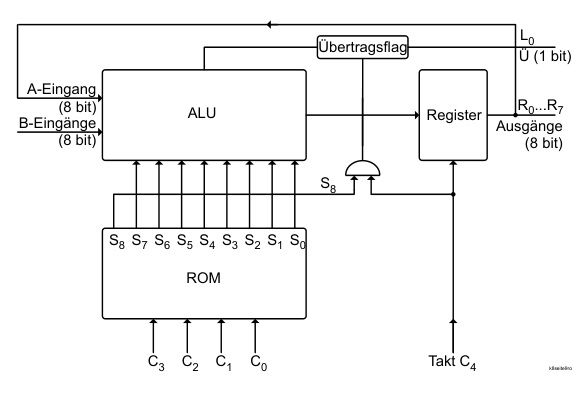
\includegraphics[width=0.8\textwidth]{akku.png}
    \captionof{figure}{Akkumulator}
    \label{fig:akku}
  \end{Figure}
  \begin{Figure}
    \centering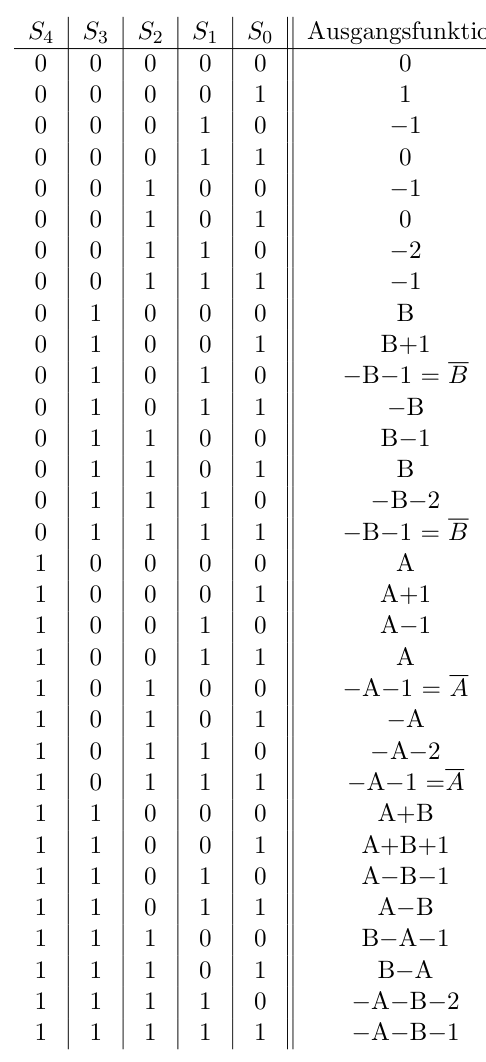
\includegraphics[width=0.7\textwidth]{addier-subtrahierwek-befehle.png}
    \captionof{figure}{8-bit Addier-Subtrahierwerk Befehle}
    \label{fig:add-sub-befehl}
  \end{Figure}
  \begin{Figure}
    \centering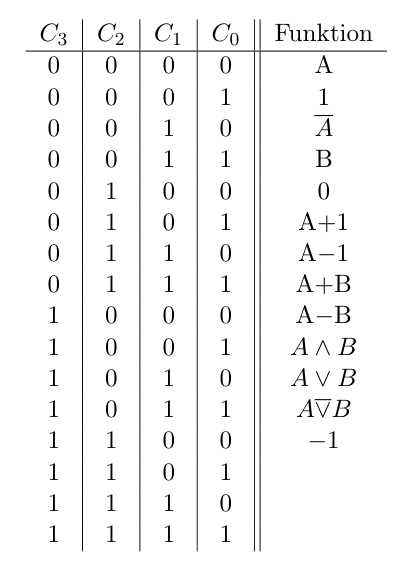
\includegraphics[width=0.7\textwidth]{sinvolle-alu-funktionen.png}
  \captionof{figure}{Sinnvolle Befehle des ALUs}
    \label{fig:alu-befehle}
  \end{Figure}
  \subsection{Akkumulator mit Datenspeicher}
  Fügt man dem Akkumulator einen Datenspeicher, hier RAM, hinzu, können jetzt auch zwischenergebnisse nicht nur abgespeichert, sondern auch wieder ausgelesen werden. Dieser ist in Abb. \ref{fig:akku-data} zu sehen.
  \begin{Figure}
    \centering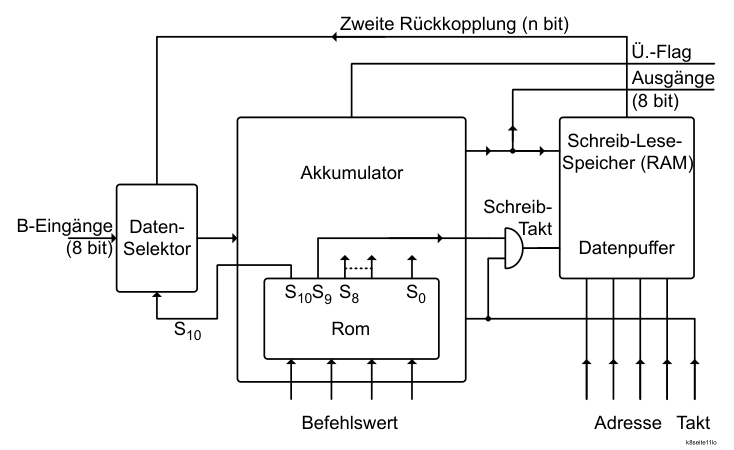
\includegraphics[width=0.8\textwidth]{akku-und-datenspeicher.png}
  \captionof{figure}{Sinnvolle Befehle des ALUs}
    \label{fig:akku-data}
  \end{Figure}
  \subsection{Prozessor}
  Um nun die Konstruktion zu einem Prozessor (Abb. \ref{fig:cpu}) zu vervollständigen, wird ein Programmspeicher mit einem Befehlszähler hinzugefügt. Aus dem Programmspeicher werden mithilfe des Befehlszählers nacheinander die Befehle des Programms aufgerufen. Ist der Befehl ausgeführt, so wird der Befehlszähler um Eins hochgeschalten. So ein Prozessor bildet der Mikroprozessor 8080.
  \begin{Figure}
    \centering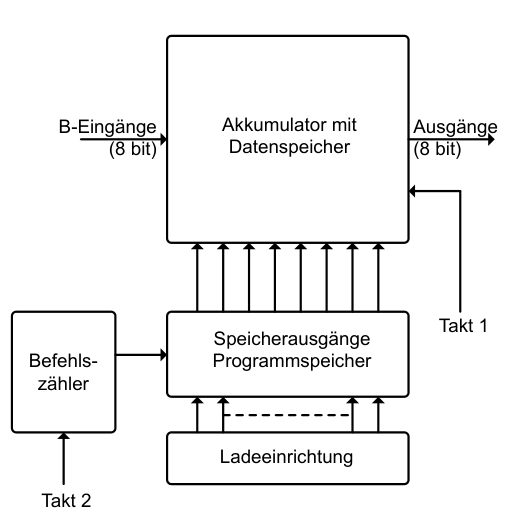
\includegraphics[width=0.8\textwidth]{cpu.png}
  \captionof{figure}{Sinnvolle Befehle des ALUs}
    \label{fig:cpu}
  \end{Figure}
	\section{Voraufgaben}
	\subsection*{A}
	Die folgenden Dualzahlen, lassen sich in die entsprechenden Hexadezimal- und Dezimalzahlen umwandeln:
	\begin{center}
		\begin{tabular}{|c|c|c|}
			\hline
			Binär               & Hexadezimal & Dezimal \\
			\hline
			1101 1111 0010 1110 & DF2E        & 57134   \\
			1111 1111           & FF          & 255     \\
			\hline
		\end{tabular}
	\end{center}
	\subsection*{B}
	Die Zahl $2115_{10}$ ist auch $1000 0100 0011_2$ oder $843_{16}$.
	\subsection*{C}
	Die Zahl $B75F_{16}$ ist auch $1011011101011111_{2}$ oder $46943_{10}$.
	\subsection*{D}
	Es können die folgenden Rechenoperationen durchgeführt weden.
	\begin{align*}
		  & 01011011 &   & 011111111 \\
		+ & 01101011 & + & 000000001 \\
		\hline
		  & 11000110 &   & 100000000 \\
	\end{align*}
	\begin{align*}
		  & 11000000 \\
		- & 10110101 \\
		\hline
		  & 00001011 \\
	\end{align*}

	Bei Zweierkomplementzahlen gibt die erste Stelle mit 1 an, ob sie negativ, oder mit 0 and, ob sie positiv ist.
	\begin{center}
		\begin{tabular}{|c|c|}
			\hline
			Zahl     & Vorzeichen \\
			\hline
			10110111 & -          \\
			11110000 & -          \\
			01111111 & +          \\
			11111111 & -          \\
			\hline
		\end{tabular}
	\end{center}
	Für die Konvertierung von einer normalen Binärzahl zu einer Zweikomplimentzahl, wird zuerst die Binär zahl invertiert und dann mit 1 addiert.
	So lassen sich subtraktion mit Zweierkomplementzahlen durch addition darstellen.
	\begin{align*}
		  & 11011011 \\
		- & 01101011 \\
	\end{align*}
	wird so zu
	\begin{align*}
		  & 11011011 \\
		+ & 10010101 \\
		\hline
		1 & 01110000 \\
	\end{align*}

	Ein Überlauf tritt dann auf, wenn zwei Zahlen addiert werden, wobei das Ergebnis größer ist, als die bereitgestellte Speichergröße. Passiert dies, wird der resultierende zusätzliche Bit nicht gespeichert und es scheint so, als ob die Zahl wieder um 1 plus die maximale Zahl, die in dem Speicher gespeichert werden kann, verringert wird.

	Eine Übetrag passiert dann, wenn bei einer Addition der nächste Bit verwendet werden muss. So führt nur die Addition von Zahlen, die an der gleichen Bit-Stelle eine 1 haben zu einem Übertrag.

	\begin{align*}
		  & 11011111 &   & 01011011         & 01011011 \\
		+ & 00111000 & - & 10111011 \hat{=} & 01000101 \\
		\hline
		1 & 00010111 &   &                  & 10100000 \\
	\end{align*}
  Bei der ersten Operation entseht ein Überlauf, wobei die Zahl mit einem 9-bit Rechner immernoch mit $-23_{10}$ immernoch im Definitionsbereich eines 8-bit Rechners wäre. Die zweite Operation ist mit $-32_{10}$ hat keinen Überlauf und ist immernoch im Definitionsbereich eines 8-bit Rechners.

  Es lassen sich auch Produkte berechnen: $1101 \cdot 1001$=1110101.

  Genauso auch Quotienten: $1110111 / 101$=10111 mit Rest 100
  \subsection*{E}
  ROM steht für Read-Only-Memory und ist ein Speicher der, wie der Name wage ahnen lässt, nur gelesen werden und nur einmal beschrieben werden kann. RAM steht für Random-Access-Memory und ist ein Speicher, der beliebig gelesen und beschrieben werden kann.
  \subsection*{F}
  Um analoge Signal in Digitale umzuwandeln benötigen wir einen DAC (Digital Analog Converter). Dieser ist durch seine Bitzahl limitiert.
  \subsection*{G}
  Ein ALU hat verschiedene logische Verknüpfungen, wie z.B. AND, OR, XOR und noch grundleregendere, wie z.B. $A+1$. Erweitert man diesen mit einem Register, einer Übertragungsflagge und einem ROM, so erhält man ein Akkumulator. Mithilfe von einer Taktung kann nun das Ergebniss gespeichert werden und ist somit kein statisches Netzwerk.
  \subsection*{H}
  Erweitert man den Akkumulator mit einem RAM und Programmspeicher, so erhält man einen vollständigen Rechner.
  \subsection*{I}
  Hat ein Rechner ein dedizierten Daten-Bus, Adressen-Bus und Steuer-Bus, so hat er eine sog. Busstruktur. Er rechnet dabei mit Bit in Binärzahlen oder Hexadezimalzahlen für die Befehle.
  \subsection*{J}
  Ein Taktzyklus durchläuft ein Takt der Clock. Ein Befehlszyklus sind alle Takte, die benötigt werden, um einen Befehl auszuführen. Ein Operationszyklus sind alle Takte, die benötigt werdne, um eine Operation durchzuführen.
  \subsection*{K}
  Der 8080-Mikroprozessor kann mit 8 Bits $2^8$ also 256 Befehle speichern. Hierbei hat jeder Befehl ein bestimmte Zahl. Diese Zahl wird Operations-Code genannt. Allerdings hat der 8080 nur 115 Befehle.
  \subsection*{L}
  Ein Zweiweg-Tri-state-Datenbus hat nicht nur die Zustände 1 und 0, sondern auch Z, der sog. hochohmige Zustand. Er signalisiert, dass es sich werder noch um 1 oder 0 handelt.
  \subsection*{M}
  Die Länge eines Befehlszyklus hängt davon ab, mit wie vielen Takten der Befehl geholt, decodiert und dann ausgeführt wird. Beim ausführen wird ein Operationszyklus durchlaufen, weshalb der Befehlszyklus auch von ihm abhängt.
  \subsection*{N}
  Der DMA (Direct Memory Access) ermöglicht den Zugriff von Befehlen auf abgespeichert Daten und kann so wiederverwendbare Ergebnisse erreichen, die sonnst erneut berechnet weden müssen. Somit wird weniger Rechenzeit beansprucht.
  \subsection*{O}
  Der Befehlszähler zählt die Befehle und weiß so die Zahl, des als nächstes auszuführenden Befehls. Der Stackpionter speichert die Adressen für abgespeicherte Werte in dem Stack.
  \subsection*{P}
  Der Stack speichert Werte von Größen, die schon zu kompilierzeit bekannt sind. Wie der Name schon suggeriert handelt es sich um ein Stapel an Befehlen. Von diesem Stapel können nur von unten oder oben Befehle hinzugefügt oder entfernt weden. So werden dort Werte die schon beim kompilieren bekannt sind dort gespeichert, sowie Werte dessen benötigte Speichergröße bekannt sind, aber erst beim Ausführen ermittelt werden, dort gespeichert. Während das Programm läuft lässt kein weiterer Speicher mehr reservieren.
  \subsection*{Q}
  Es gibt die volgenden Adressierungsarten:
  Unmittelbare Adressierung: Der Befehl hat den Wert selber.
  Direkte Adressierung: Der Befehl kennt direkte Adresse des Werts.
  Indirekt Adressierung: Der Befehl kennt die Adresse des Werts durch den Stackpointer.
  Relative Adressierung: Der Befehl kennt durch das Addieren von einer bestimmten Größe die Adresse in Abhängigkeit eines Ausgangpunktes (Arrays auf dem Stack).
  Indizierte Adressierung: Der Befehl kennt durch Indexen die Adressen einer Reihe an Werten.
  \subsection*{R}
  Der 8080 hat die folgenden Operationszyklen Befehlsaufruf, Speicher lesen, Speicher schreiben, Stack lesen, Stack einschreiben, Eingabe, Ausgabe, Unterbrechung und halten.
  \subsection*{S}
  Der erste Operationszyklus liest den Befehl ein, damit er dann mit dem Befehlregister decodiert werden kann.


  
	\section{Auswertung}
	\section{Fazit}
\end{multicols}
\end{document}
